\documentclass{TDP003mall}
\usepackage{graphicx}
\graphicspath{ {bilder/} }
\usepackage{enumitem}
\setlist[description]{leftmargin=\parindent,labelindent=\parindent}

\newcommand{\version}{Version 1.0}
\author{Love Bäckman, \url{lovba497@student.liu.se} \\
  Gustav P Svensson, \url{gussv375@student.liu.se}}
\title{Kravspecifikation}
\date{2016-11-27}
\rhead{Love Bäckman\\
Gustav P Svensson}



\begin{document}
\projectpage

\tableofcontents
\newpage

\section{Revisionshistorik}
\begin{table}[!h]
\begin{tabularx}{\linewidth}{|l|X|l|}
\hline
Ver. & Revisionsbeskrivning & Datum \\\hline
0.1 & Ett första utkast & 161110 \\\hline
1.0 & Komplettering & 161127 \\\hline
\end{tabularx}
\end{table}


\section{Spelide}
X Runner är ett utmanade plattformsracingspel som utspelar sig i en 2D-värld.
Spelarens utmaning är att så snabbt som möjligt ta sig till målområdet, men inte utan att beakta farorna som lurar på vägen. Klarar spelaren av att undvika dem, eller rent av utnyttja dem till sin fördel, på sin väg mot rekordet?

\section{Målgrupp}
Spelets målgrupp är personer i alla åldrar som gillar utmanande plattformsracingspel likt Pixelvania.

\section{Spelupplevelse}
X Runner försöker mätta spelarens omättbara tävlingslystnad genom att ständigt utmana spelaren fram tills dess att denne konsekvent kan uppnå det ultimata målet, ``perfect runs''.

\section{Konventioner}
\begin{itemize}
\item Med NPC åsyftas ickespelarkaraktärer.
\item Med objekt åsyftas samtliga typer av spelare, NPC's och block.
\item Med specialblock åsyftas samtliga typer av block, exklusive Terrain.
\item Referering till annan plats i dokumentet sker på formen \textbf{Sektionsrubrik(x.y)[a,b,...]}.
\\\\
Exempel: \textbf{Regler(5.1)[1,2]} hänvisar till listföremål nummer 1 och 2 under den första underrubriken under den femte underrubiken under sektionsrubriken \textbf{Regler}, det vill säga listföremålen ``Slow Birds är icke-solida'' och ``Slow Birds påverkas inte av gravitation''.
\item Referering till krav sker på formen \textbf{Krav(x,y,...)}.
\end{itemize}

\newpage

\section{Spelmekanik}
\subsection{Meny}
I menyn kan spelaren starta en bana eller avsluta spelet. Menyval görs genom klick med muspekaren eller piltangenterna följt av Enter. \textit{(I mån av tid, online-multiplayer: spelaren ska kunna starta en nätverks-session med andra spelare.)}

\subsection{In-game}

\subsubsection{Spelarkontroller}
\begin{tabular}{|c|c|}
\hline
\textbf{Knapptryck} & \textbf{Händelse} \\\hline
W eller $\uparrow$ & Spelaren hoppar \\\hline
A eller $\leftarrow$ & Spelaren går åt vänster \\\hline
D eller $\rightarrow$ & Spelaren går åt höger \\\hline
ESC & Återgå till menyn \\\hline
\end{tabular}

\subsubsection{Spelarkollision med NPC's \& specialblock}
\\\\
\begin{tabular}{|l|l|}
\hline
\textbf{NPC / Specialblock} & \textbf{Händelse vid kollision med spelare}\\\hline
Slow Bird & Spelarens hastighet minskar i ett antal sekunder\\\hline
Boost Bird & Spelarens hastighet ökar i ett antal sekunder\\\hline
Bomb from Bomb bird Bird & Spelaren kan inte röra sig i ett antal sekunder, Bomb from Bomb bird de-spawnar\\\hline
Quicksand & Spelarens hastighet minskar och spelaren kan inte hoppa \\\hline
Goalblock & Banan är avklarad \\\hline
\end{tabular}

\subsubsection{Online-multiplayer (i mån av tid)}
Online-multiplayer innebär att spelare kan starta en nätverks-session med andra spelare och tävla mot varandra på en bana. Till en början implementeras detta enbart för lokala nätverk med en spelare som agerar host. 

\subsubsection{Rendering}
Den renderade delen av banan ska förflytta sig så att spelaren alltid är centrerad på skärmen.

\newpage

\section{Regler}

\subsection{Avklarande av banor}
\begin{enumerate}
\item När spelaren kommit i mål (kolliderat med ett goalblock) är banan avklarad och spelaren återgår till menyn. \textit{(I mån av tid, online-multiplayer: Spelaren återgår till menyn efter att ett antal sekunder har gått sedan den förste spelaren kommit mål. Om alla spelare kommit i mål återgår spelaren direkt till menyn.}
\item Om spelaren slog den nuvarande rekordtiden för banan kommer dennes tid att sparas som den nya rekordtiden. \textit{(Lokal funktion, påverkas inte av att online-multiplayer eventuellt implementeras.)}
\end{enumerate}

\subsection{Soliditet}
\begin{enumerate}
\item Inga objekt kan passera genom ett solidt objekt.
\end{enumerate}

\subsection{Gravitation}
\begin{enumerate}
\item Att ett objekt påverkas av gravitation innebär att objektet faller sålänge de inte befinner sig ovanpå ett solidt objekt. Fallhastigheten skall antingen vara konstant eller baseras på ett objekts viktattribut, valet görs vid implementation.
\end{enumerate}

\subsection{Spelare}
\begin{enumerate}
\item Spelaren är icke-solid.

\item Spelaren påverkas av gravitation.

\item Spelaren kan röra sig i sidled såvida denna rörelse inte innebär kollision med ett solidt objekt. Spelaren kan röra sig i sidled även om denne faller.

\item Om spelaren står på ett solidt objekt kan denne hoppa. Vid kollision med ett solidt objekt ovanför spelaren avbryts hoppet och spelaren börjar falla till följd av gravitationen.

\item Om spelaren kolliderar med en NPC eller ett specialblock utförs händelserna specificerade under \textbf{Spelmekanik(2.2)}.

\item \noindent\textit{(I mån av tid: walljumping)} Walljumping kan utföras om spelaren efter kollision med en vägg utför ett nytt hopp om denne fortfarande har kontakt med väggen och inte redan börjat falla nedåt.

\newpage

\item \noindent\textit{(I mån av tid: hoppa för hastighet)} För öka att sin hastighet kan spelaren hoppa med sidledsrörelse flera på varandra efterföljande gånger utan att kollidera med ett solidt block.
\\\\
I \textbf{figur 1} nedan visualiseras hur implementation är tänkt att fungera. Som synes både påbörjar samt avslutar spelaren det första hoppet med sidledsrörelse och erhåller således bonushastighet till nästa hopp (vilket också innebär att spelaren hoppar högre).
\\\\
I den första bilden utför sedan spelaren ytterligare ett hopp med sidledsrörelse, och erhåller således ytterligare bonushastighet till ett eventuellt tredje hopp. 
\\\\
I den andra bilden kolliderar istället spelaren med ett solidt block under sitt andra hopp, vilket får till följd att spelaren tappar all bonushastighet.
\\\\
Samtliga sätt som spelaren kan förlora bonushastigheten på är:
\begin{itemize}
\item Spelaren kolliderar med ett solidt objekt (landning ignoreras)
\item Spelaren har ingen sidledsrörelse i början av hoppet, det vill säga spelaren hoppar rakt upp.
\item Spelaren har ingen sidledsrörelse vid landning, det vill säga spelaren faller rakt nedåt i landningsögonblicket.
\item Spelaren slutar hoppa.
\end{itemize}
\end{enumerate}

\begin{figure}[!h]
  \centering
  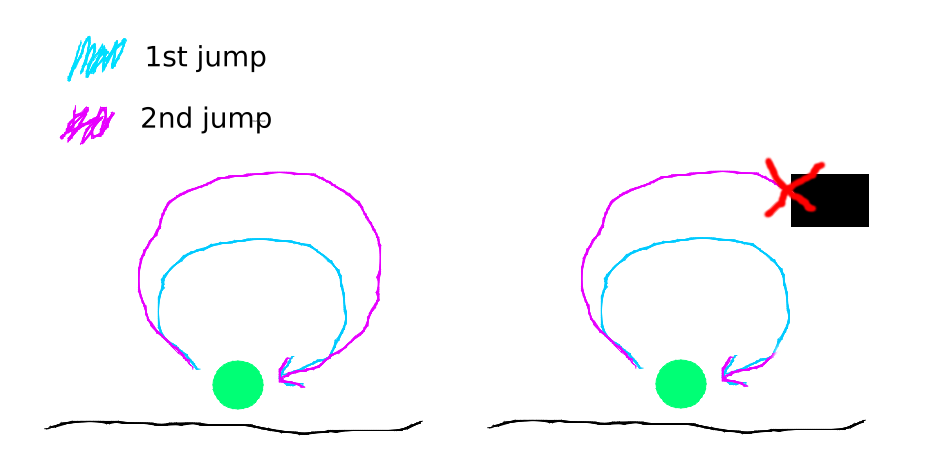
\includegraphics[scale=0.5]{speed_jump}
  \caption{Hoppa för hastighet}
  \label{Meny}
\end{figure}

\newpage

\subsection{NPC's}
Se \textbf{Spelmekanik(2.2)} för händelser vid kollision mellan NPC's och spelare.

\subsubsection{Bomb Bird}
\begin{enumerate}
\item Bomb Birds är icke-solida.
\item Bomb Birds påverkas inte av gravitation.
\item Bomb Birds kan endast röra sig i sidled \textit{(i mån av tid: kan endast röra sig i sidled utefter en sinuskurva)}.
\item När en Bomb Bird kolliderar med ett solidt objekt byter den riktning i sidled.
\item Bomb Birds spawnar efter en utsatt tid, beroende på vilken bana spelaren spelar.
\item Inom ett utsatt interval spawnar Bomb birds en bomb, Bomb from Bomb bird.
\end{enumerate}

\subsubsection{Boost Bird}
\begin{enumerate}
\item Boost Birds är icke-solida.
\item Boost Birds påverkas inte av gravitation.
\item Boost Birds kan endast röra sig i sidled \textit{(i mån av tid: kan endast röra sig i sidled utefter en sinuskurva)}.
\item När en Boost Bird kolliderar med ett solidt objekt byter den riktning i sidled.
\item Boost Birds spawnar efter en utsatt tid, beroende på vilken bana spelaren spelar.
\end{enumerate}

\subsection{Block}
Se \textbf{Spelmekanik(2.2)} för händelser vid kollision mellan specialblock och spelare.

\subsubsection{Bomb from Bomb Bird}
\begin{enumerate}
\item Bomb from Bomb Bird är icke-solidt.
\item Bomb from Bomb Bird påverkas av gravitation.
\item När Bomb from Bomb Bird spawnas av en Bomb Bird faller det nedåt till följd av gravitationen. Efter att det kolliderat med ett solidt block ligger det kvar i ett antal sekunder innan det despawnar eller tills dess att en spelare kolliderat med bomben.
\end{enumerate}

\subsubsection{Quicksand}
\begin{enumerate}
\item Quicksand är solidt.
\item Quicksand påverkas inte av gravitation.
\end{enumerate}

\subsubsection{Goalblock}
\begin{enumerate}
\item Goalblock är icke-solidt.
\item Goalblock påverkas av gravitation.
\end{enumerate}

\subsubsection{Terrain}
\begin{enumerate}
\item Terrain är solidt.
\item Terrain påverkas inte av gravitation.
\end{enumerate}

\section{Visualisering}
\begin{figure}[!h]
  \centering
  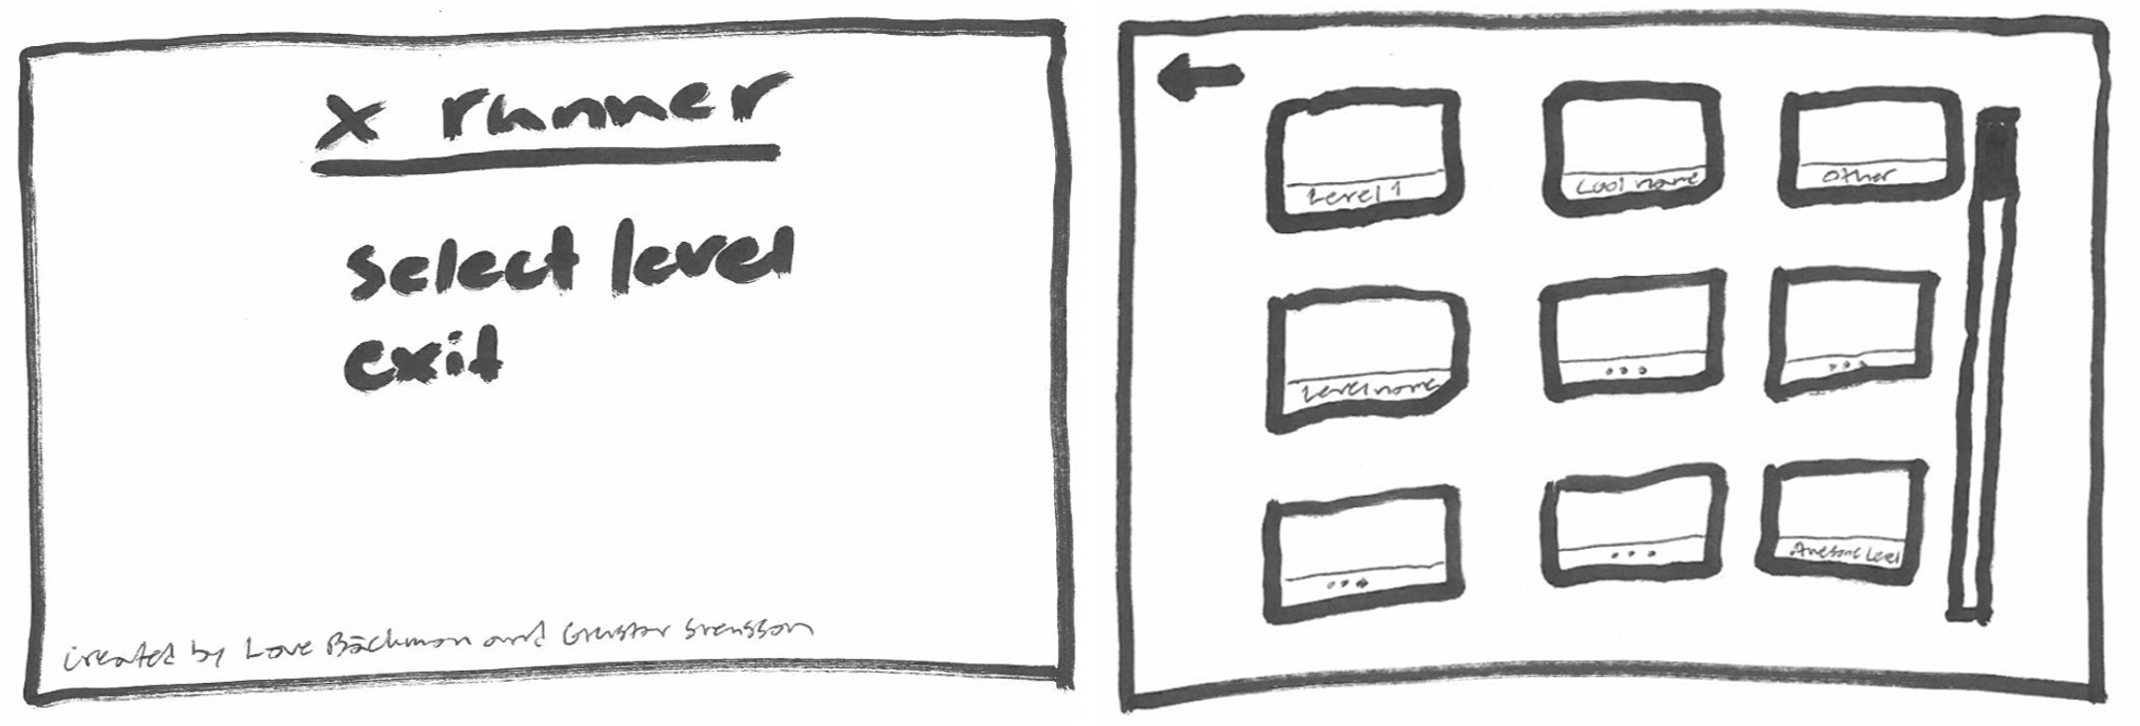
\includegraphics[scale=0.20]{startmeny}
  \caption{Meny}
  \label{Meny}
\end{figure}



\begin{figure}[!h]
  \centering
  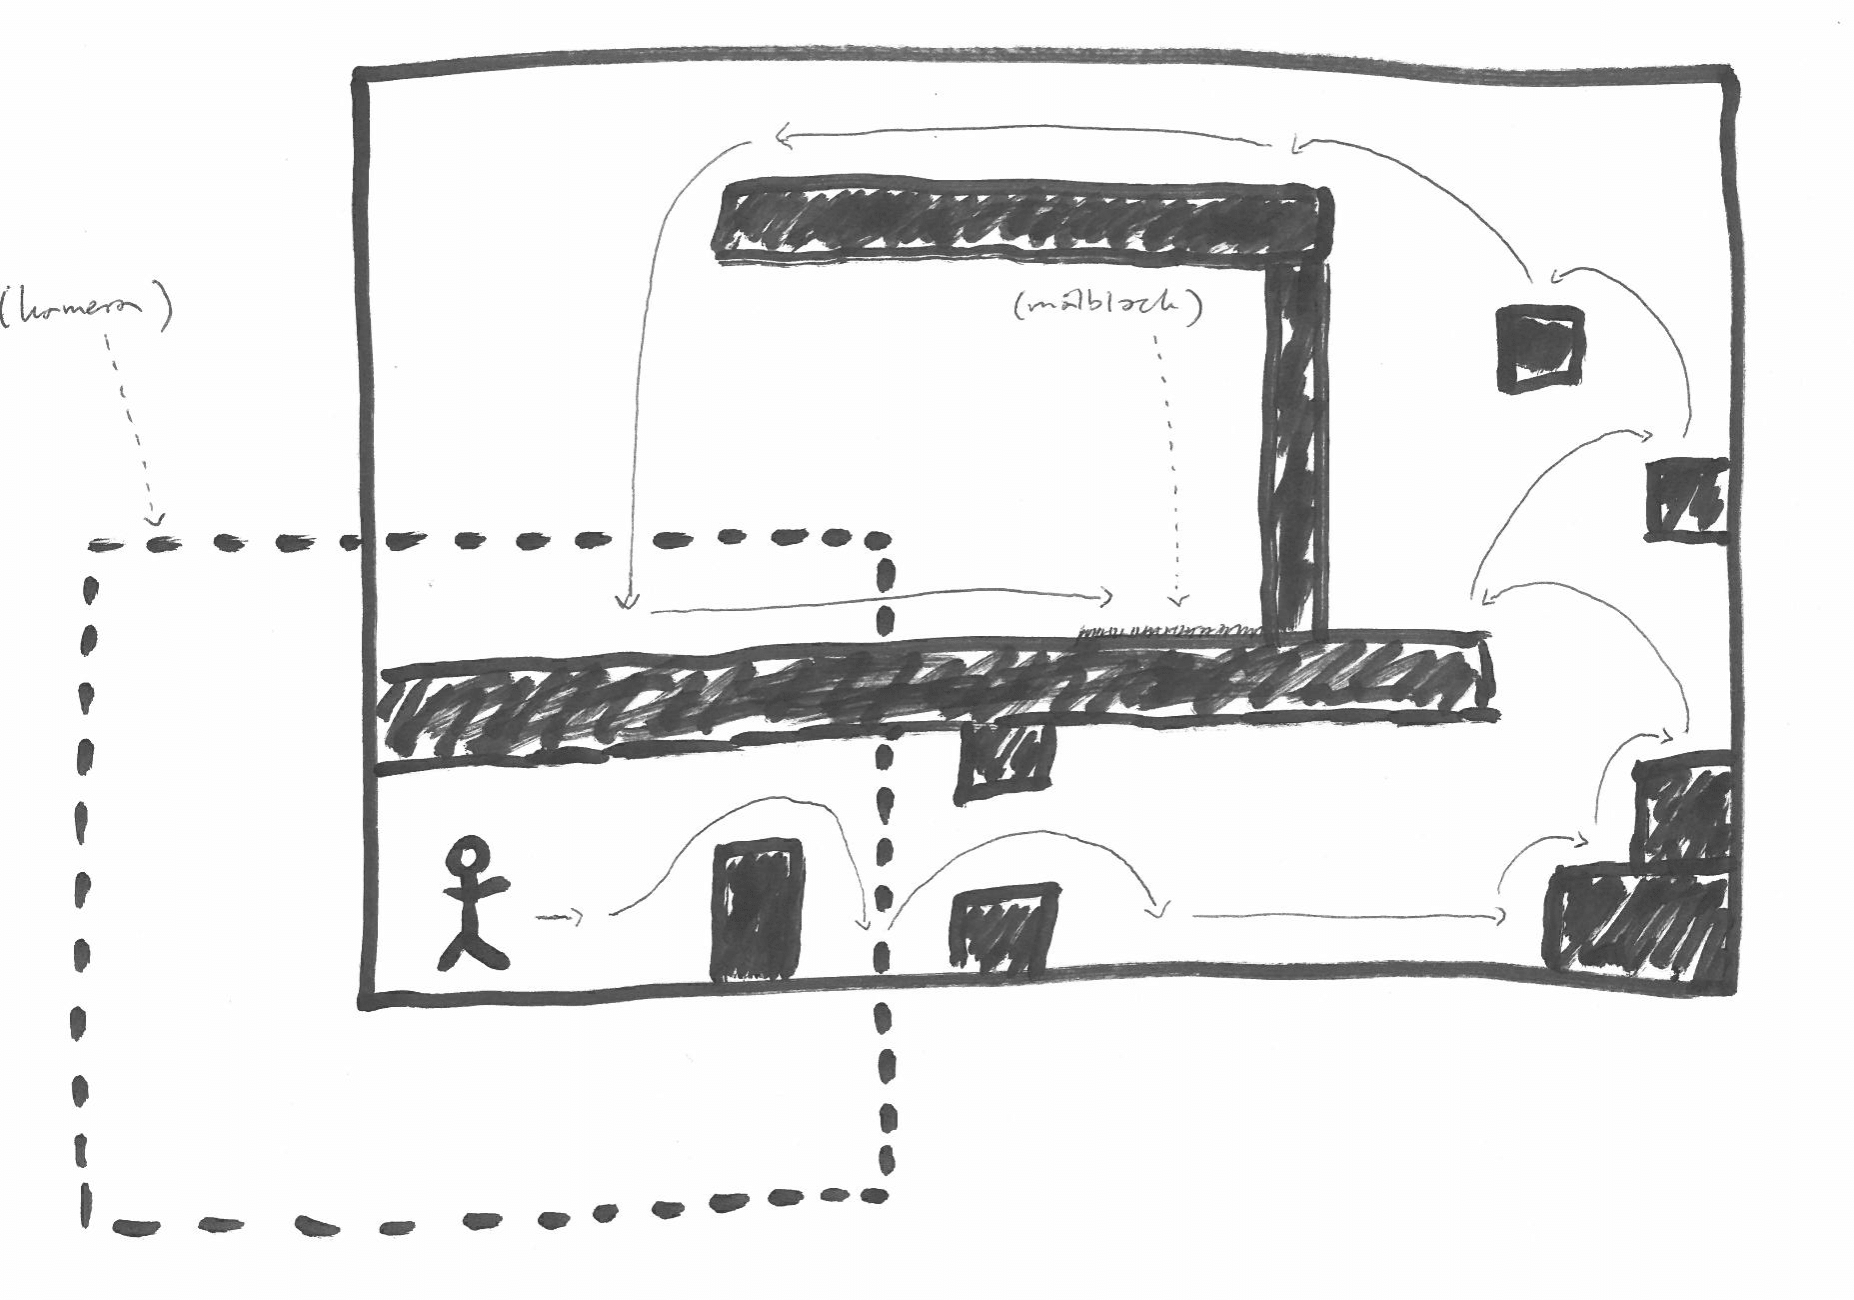
\includegraphics[scale=0.20]{spelplan}
  \caption{Spelplan}
  \label{Spelplan}
\end{figure}

\section{Kravformulering}
\subsection{Ska-krav}
\begin{description}
\item[1] Det ska finnas minst ett spelarobjekt på den aktiva banan.
\item[2] Spelaren ska kunna förflytta sig i sidled samt hoppa med tangentbordet enligt specificerade restriktioner (\textbf{Spelmekanik(2.1)}, \textbf{Regler(4)[3,4]})
\item[3] Aktiv bana ska renderas tvådimensionellt på skärmen centrerat runt spelaren (\textbf{Spelmekanik(2.3)}, \textbf{Visualisering(Figur 4)})
\end{description}

\subsection{Bör-krav}
\begin{itemize}
\item[4] Objekt ska påverkas av gravitation om det specificerats för objektet (\textbf{Regler(3)[1]})
\item[5] Kollision mellan objekt ska påverkas av soliditet (\textbf{Regler(2)[1]})
\item[6] Det ska kunna finnas flera NPC's och specialblock på den aktiva banan.
\item[7] NPC's och specialblock ska kunna spawnas dynamiskt (\textbf{Regler(5.1)[5]}, \textbf{Regler(5.2)[5,6]})
\item[8] NPC's ska röra sig enligt specificerade restriktioner (\textbf{Regler(5.1)[3]}, \textbf{Regler(5.2)[3]})
\item[9] Rekordtiden för varje bana ska sparas (\textbf{Regler(1)[2]})
\item[10] Rekordtiden för den aktiva bana ska renderas på skärmen.
\item[11] Spelaren ska kunna walljumpa (\textbf{Regler(4)[6]})
\item[12] Spelarens ska kunna hoppa för hastighet (\textbf{Regler(4)[6]})
\item[13] När spelaren kolliderar med en NPC eller ett specialblock utförs de specificerade kollisionshändelserna (\textbf{Spelmekanik(2.2)})
\item[14] Menyn ska renderas tvådimensionellt på skärmen (\textbf{Visualisering(Figur 2)}, \textbf{Visualisering(Figur 3)})
\item[15] Spelaren ska kunna interagera med menyn (\textbf{Spelmekanik(1)})
\item[16] Det ska vara möjligt att spela online multiplayer (\textbf{Spelmekanik(2.1)}, \textbf{Spelmekanik(2.3)}, \textbf{Regler(1)[1]})
\end{itemize}

\section{Kravuppfyllelse}
\textit{Spelet ska simulera en värld som innehåller olika typer av objekt. Objekten ska ha olika beteenden och röra
sig i världen och agera på olika sätt när de möter andra objekt.}
\begin{itemize}
\item Varje bana har flera olika typer av block och NPC's med olika beteenden och egenskaper. De interagerar även med varandra och spelaren och vissa av dem rör sig (\textbf{Krav(2,4,5,8,13)})
\end{itemize}


\noindent\textit{Det måste finnas minst tre olika typer av objekt och det ska finnas flera instanser av minst två av dessa.
T.ex ett spelarobjekt och många instanser av två olika slags fiendeobjekt.}
\begin{itemize}
\item Det kommer finnas flera olika yper av block och NPC's samt minst en spelarkaraktär på varje bana (\textbf{Krav(1,6)})
\end{itemize}

\noindent\textit{Ett beteende som måste finnas med är att figurerna ska röra sig över skärmen. Rörelsen kan följa ett
mönster och/eller vara slumpmässig. Minst ett objekt, utöver spelaren ska ha någon typ av rörelse.}
\begin{itemize}
\item Spelarkaraktären kommer kunna röra sig i sidled samt hoppa (\textbf{Krav(2)})
\item NPC's kommer röra sig i sidled efter ett fördefinierat mönster (\textbf{Krav(8)})
\item Vissa objekt kommer påverkas av gravitation (\textbf{Krav(4)})
\end{itemize}

\noindent\textit{En figur ska styras av spelaren, antingen med tangentbordet eller med musen. Du kan även göra ett spel där
man spelar två stycken genom att dela på tangentbordet (varje spelare använder olika tangenter). Då styr
man var sin figur.}
\begin{itemize}
\item Spelaren kommer styra sin karaktär genom att använda tangentbord (\textbf{Krav(2)})
\end{itemize}

\noindent\textit{Grafiken ska vara tvådimensionell.}
\begin{itemize}
\item Vi använder 2D-grafik med hjälp av SFML (\textbf{Krav(3,14)})
\end{itemize}

\noindent\textit{Världen (spelplanen) kan antas vara lika stor som fönstret (du kan göra en större spelplan med scrollning,
men det blir lite krångligare).}
\begin{itemize}
\item Spelplanen kommer använda scrolling så att spelaren alltid är centrerad på skärmen (\textbf{Krav(3)})
\end{itemize}

\textit{Det ska finnas kollisionshantering, det vill säga, det ska hända olika saker när objekten möter varandra, 
de ska påverka varandra på något sätt. T.ex kan ett av objekten tas bort, eller så kan objekten förvandlas på
något sätt, eller så kan ett nytt objekt skapas.}
\begin{itemize}
\item Olika händelser kommer ske vid kollision mellan olika objekt (\textbf{Krav(2,5,8,13)})
\end{itemize}

\noindent\textit{Spelet måste upplevas som ett sammanhängande spel som går att spela!}
\begin{itemize}
\item Ja, det kommer det att göra (\textbf{Krav(null)})
\end{itemize}

\end{document}
